\chapter{Présentation 1}  

Un logiciel de présentation permet de bâtir des diapositives à partir de gabarits de départ qui seront ensuite personnalisés. Ces diapositives s'enrichissent de textes, de vidéos et de mises en forme divrses.

\section*{Synoptique}

{\footnotesize
\begin{itemize}
\item Logiciel \emph{Microsoft PowerPoint} 
\item Matières concernées : titulaire.
\item Compétences : 
        \begin{itemize}
        \item créer une diapositive à partir d'un modèle ; 
	\item créer une diapositive à partir d'une diapositive vide ;
	\item insérer un texte ;
	\item insérer une image ;
	\item insérer une image d'arrière-plan ;
	\item utiliser la trieuse de diapositive ;
	\item utiliser les notes de présentation ;
	\item imprimer les diapositives ;
	\item exporter les diapositives au format \texttt{PDF}.
        \end{itemize}
\item Cette fiche est à réaliser :
        \begin{itemize}
        \item avant les vacances de février. 
        \end{itemize}
\end{itemize}
}% fin du footnotesize


\vfill
\phantom{rien}

%
%
% SEANCE  1
%
%

\pagebreak

\section{Séance 1 : une présentation}\label{fichePresentation6e1}

\subsection{Pour bien démarrer...}

Dès que vous avez ouvert un nouveau document dans \emph{PowerPoint}, sauvegardez-le au format Nom-seance1.pptx : dans le menu \texttt{Fichier}, choisir \texttt{Enregistrer sous}.

\uneimageici{./images/generales/clavierCmdS}{.4\textwidth}


\subsection{Sujet de l'activité...}

\boiteEnonceLarge{Le but de cette séance est créer une présentation sur un thème communiqué par votre enseignant à l'aide du logiciel \emph{Microsoft PowerPoint} et qui utilise tous les points ci-dessous :
\begin{itemize}
	\item une diapositive de titre avec votre nom,
	\item des diapositives de différents styles (texte, image avec texte, image seulement, ...),
	\item des animations entre les diapositives et sur chaque diapositive,
	\item un arrière-plan utilisant une image,
	\item une diapositive de fin avec remerciements,
	\item des notes.
\end{itemize}
\vspace{8pt}
Une fois votre travail terminé, exportez votre présentation au format PDF et enregistrez-le sur votre ordinateur avant de l'envoyer sur \emph{Teams}, à endroit indiqué par votre enseignant.
}% fin énoncé

\textbf{Pour obtenir de l'aide, rendez-vous à la page suivante.}

\subsection{Pour aller plus loin...}

Insérer une vidéo dans votre présentation.



%\vfill

%\cadre{Pensez à sauver régulièrement votre travail en appuyant sur \texttt{Cmd + S} ou à partir du menu \texttt{Fichier} en choisissant \texttt{Enregistrer}.

%\uneimageici{./images/generales/clavierCmdS}{.3\textwidth}



\newpage

\section{Aide pour réaliser l'activité}\label{aidePresentation}

\subsection{Les ingrédients d'une bonne présentation}

Une présentation orale peut s'appuyer sur un diaporama qui permet d'illustrer les propos de l'orateur et lui permet de garder un fil conducteur. Attention, le diaporama est bien une illustration du discours : l'orateur ne doit jamais lire le contenu des diapositives. D'ailleurs les diapositives ne doivent pas contenir de phrase mais seulement des mots-clés, des graphiques, des schémas et des illustrations. Le diaporama ne doit pas entrer en concurrence avec l'orateur, qui doit concentrer l'attention du public.

\subsubsection{Mise en forme du diaporama}

\begin{itemize}
\item Choisir une ligne graphique simple, épurée, identique sur chaque diapositive.
\item Utiliser une police de caractère simple (type Arial ou Times) et de grande taille (par ex. 32 pour les textes et 44 pour les titres). Garder la même police partout.
\item Utiliser des couleurs vives à fort contraste avec le fond (texte foncé sur fond clair). Éviter les textes clairs sur fond noir qui ne se voient pas si la salle n'est pas suffisamment sombre.
\item Numéroter chaque diapositive.
\item Utiliser un minimum d'animations : elles font perdre l'attention de l'auditoire, voire l'agacent.
\item Écrire le minimum de texte : se limiter à quelques mots-clés.
\end{itemize}

\subsubsection{Contenu du diaporama}

\begin{itemize}
\item Première diapositive : titre, prénom, nom, date et une illustration. C'est la diapositive qui est affichée avant même le début de la présentation. L'auditoire doit savoir qui va parler et ce qu'il va présenter.
\item Seconde diapositive : le plan de la présentation.
\item Avant-dernière / dernière diapositive : conclusion et, si nécessaire, remerciements.
\item Entre la diapositive de titre et celle de conclusion, enchaînement logique de diapositives suivant un plan bien défini. Il faut raconter une histoire !
\end{itemize}

\subsubsection{Deux exemples}

Comment présenter l'Institut Florimont ? Ci-dessous, à gauche, une mauvaise diapositive contenant beaucoup de texte. À droite, une diapositive visuellement agréable qui ne contient que les chiffres clés et quelques icônes pour que l'orateur se souvienne de ce qu'il doit dire.

\deuximagesici{./images/presentation/diapoBad}{\textwidth}{./images/presentation/diapoGood}{\textwidth} 



\subsection{Les outils dont vous aurez besoin}\label{Presentation6eOutils}

Les nouveaux outils dont vous aurez besoin pour réaliser les trois séances sur la création d'une présentation sont décrits ci-dessous :


\begin{itemize}   
\item \textbf{créer une nouvelle présentation}, voir section \vref{Presentation1new} ;
\item créer \textbf{une diapositive à partir d'un modèle}, voir section \vref{Presentation1diapoModele} ;
\item utiliser la \textbf{trieuse de diapositives (ordonner, dupliquer et supprimer les diapositives)}, voir section \vref{Presentation1trieuse} ;
\item \textbf{ajouter une diapositive}, voir section \vref{Presentation1nouvelleDiap} ;
\item créer une \textbf{diapositive à partir d'une diapositive vide}, voir section \vref{Presentation1DiapoSansModele} ;
\item \textbf{insérer un texte dans une diapositive}, voir section \vref{Presentation1texte} ;
\item \textbf{insérer une image dans une diapositive}, voir section \vref{Presentation1image} ;
\item \textbf{définir une image d'arrière-plan}, voir section \vref{Presentation1imageFond} ;
\item \textbf{utiliser les animations}, voir section \vref{Presentation1effets} ;

\item \textbf{ajouter des notes de présentations}, voir section \vref{Presentation1notes} ;
\item \textbf{imprimer une présentation et ses notes}, voir section \vref{Presentation1export} ;
\item \textbf{exporter une présentation au format \texttt{PDF}}, voir section \vref{Presentation1exportPDF} 
\end{itemize}  





\subsubsection{Créer une nouvelle présentation}\index{Impress!Créer présentation}\index{Créer présentation (Impress)}\label{Presentation1new}

Ouvrez le navigateur web et allez sur \texttt{office.com}. Cliquez sur le bouton \texttt{Connexion}.

\uneimageici{./images/tableur/ecran_office_com_crop}{.5\textwidth}

Cela ouvre la page de connexion de l'Institut. Entrez votre identifiant et votre mot de passe pour accéder au portail d'office.com. Vous trouverez sur la gauche les boutons menant à toutes les applications d'office. Cliquez sur le logo de \emph{PowePoint}. Cliquez ensuite sur le cadre blanc avec la croix orange pour ouvrir une fenêtre de travail \emph{PowePoint}.

\uneimageici{./images/presentation/ecran_office_PP_crop}{.45\textwidth}





\subsubsection{Une diapositive à partir d'un modèle}\index{Impress!Diapositive à partir modèle}\index{Diapositive à partir modèle (Impress)}\label{Presentation1diapoModele}

Pour créer une diapositive, il faut cliquer sur le bouton \texttt{Nouvelle diapositive}, en haut à gauche de l'espace de travail \circled{1}. S'ouvre alors une liste de modèles, comme présenté ci-dessous. Choisissez le modèle \texttt{Contenu avec légende} en cliquant dessus \circled{2}.

\uneimageici{./images/presentation/Impress_02Creer_01_OPP_crop}{.5\textwidth}



La diapositive est ensuite ajoutée à la présentation.

\uneimageici{./images/presentation/Impress_02Creer_02_OPP_crop}{.6\textwidth}

Ce modèle permet l'insertion très facile de textes et d'images (ou d'autres types de contenu).

% \uneimageici{./images/presentation/Impress_02Creer_02}{.6\textwidth}

\paragraph{Insérer un texte} en cliquant sur le cadre de texte

Cliquez sur le cadre de gauche, dans lequel il est écrit \texttt{Click to add text} (en français : Cliquez pour ajouter du texte). Vous pouvez ensuite immédiatement écrire du texte pour cette partie de la diapositive.

Pour mettre en forme le texte, il faut se rendre à l'onglet Accueil \circled{1}. Les différentes options sont ensuite disponibles en haut de la fenêtre \circled{2}.

\uneimageici{./images/presentation/Impress_02Creer_03_OPP_crop}{\textwidth}




\paragraph{Insérer une image} en cliquant sur l'icône en bas à gauche des options proposées, comme représenté ci-dessous :

\uneimageici{./images/presentation/Impress_03Inserer_01_OPP_crop}{.3\textwidth}

Dans la boîte de dialogue qui s'ouvre, rechercher le fichier qui contient l'image à insérer et terminer en appuyant sur le bouton \texttt{Insérer}.

\vspace{1em}

L'image peut être redimensionnée et tournée :\label{poigneeTourneZoom} 

\begin{itemize}
\item pour \textbf{redimensionner l'image}, cliquer une fois dessus et utiliser les \textbf{poignées} qui apparaissent \circled{1} ;
\item pour effectuer une \textbf{rotation de l'image}, cliquer une fois dessus et utiliser la \textbf{poignée de rotation} qui apparait en haut \circled{2}.
\end{itemize}

\uneimageici{./images/presentation/Impress_03Inserer_02_OPP_crop}{.5\textwidth}

À tout moment il est possible de passer d'un modèle de diapositive à un autre modèle en allant dans l'onglet \texttt{Accueil} \circled{1} puis en cliquant sur \texttt{Disposition} \circled{2}. On remarque alors que l'image et le texte précédemment insérés sont conservés.

\uneimageici{./images/presentation/Impress_03Inserer_03_OPP_crop}{.8\textwidth}



\subsubsection{Trieuse de diapositives (ordonner, dupliquer et supprimer les diapositives)}\index{Impress!Trieuse de diapositive}\index{Trieuse de diapositive (Impress)}\index{Impress!Dupliquer une diapositive}\index{Impress!Ordonner les diapositives}\index{Ordonner les diapositives (Impress)}\index{Impress!Dupliquer une diapositive}\index{Dupliquer une diapositive (Impress)}\index{Impress!Supprimer une diapositive}\index{Supprimer une diapositive (Impress)}\label{Presentation1trieuse}

La trieuse de diapositives est un affichage de l'ensemble de la présentation qui permet de distinguer toutes les diapositives, de naviguer rapidement d'une à l'autre et de les déplacer, de les dupliquer ou encore de les supprimer.

Pour y accéder, il faut choisir l'onglet \texttt{Affichage} \circled{1} puis cliquer sur \texttt{Trieuse de diapositives} \circled{2}.

\uneimageici{./images/presentation/Impress_05Trieuse_01_OPP_crop}{.7\textwidth}

\begin{itemize}
	\item Pour retourner dans la vue normale d'une diapositive, il suffit de double-cliquer dessus ;
	\item Pour déplacer une diapositive, il suffit de cliquer dessus et de maintenir le bouton de souris enfoncé tout en la déplaçant. Relachez le bouton de souris quand la diapositive se trouve où vous le voulez;
	\item Pour dupliquer une diapositive, on peut faire un clic droit dessus et sélectionner \texttt{Dupliquer la diapositive}. ;
	\item Pour supprimer une diapositive, on peut faire un clic droit dessus et sélectionner \texttt{Supprimer la diapositive} ou simplement appuyer sur la touche \texttt{Effacer} (la flèche pointant vers la gauche, au-dessus de la touche \texttt{Entrer}).
\end{itemize}




\subsubsection{Ajouter une diapositive}\index{Impress!Créer diapositive}\index{Diapositive, créer (Impress)}\label{Presentation1nouvelleDiap}

Pour ajouter une diapositive, deux solutions sont possibles :

\begin{itemize}
\item Un clic droit sur une zone vide de la trieuse permet d'insérer une nouvelle diapositive à cet endroit ou de coller une diapositive précédemment copiée à l'aide de \texttt{Cmd + C} (figure à gauche) ; 
\item un clic droit sur une diapositive dans la trieuse permet de choisir d'appliquer les options précédentes comme si on avait cliqué juste après cette diapositive ou de dupliquer la diapositive sélectionnée (figure ci-dessous à droite).
\end{itemize}
	
\deuximagesici{./images/presentation/Impress_04NouvelleDia_02_OPP_crop}{.7\textwidth}
	      {./images/presentation/Impress_04NouvelleDia_03_OPP_crop}{.7\textwidth}



\subsubsection{Diapositive à partir d'une diapositive vide}\index{Impress!Diapositive sans modèle}\index{Diapositive à partir d'une diapositive vide (Impress)}\label{Presentation1DiapoSansModele}


%\begin{minipage}[c]{.58\textwidth}
Si aucun des modèles proposés ne convient à ce que l'on souhaite réaliser, on peut partir d'une diapositive vide. Par exemple, la diapositive montrée sur la figure ci-dessous est réalisée à partir d'une diapositive vide plutôt qu'à partir d'un modèle.

%\centering%
%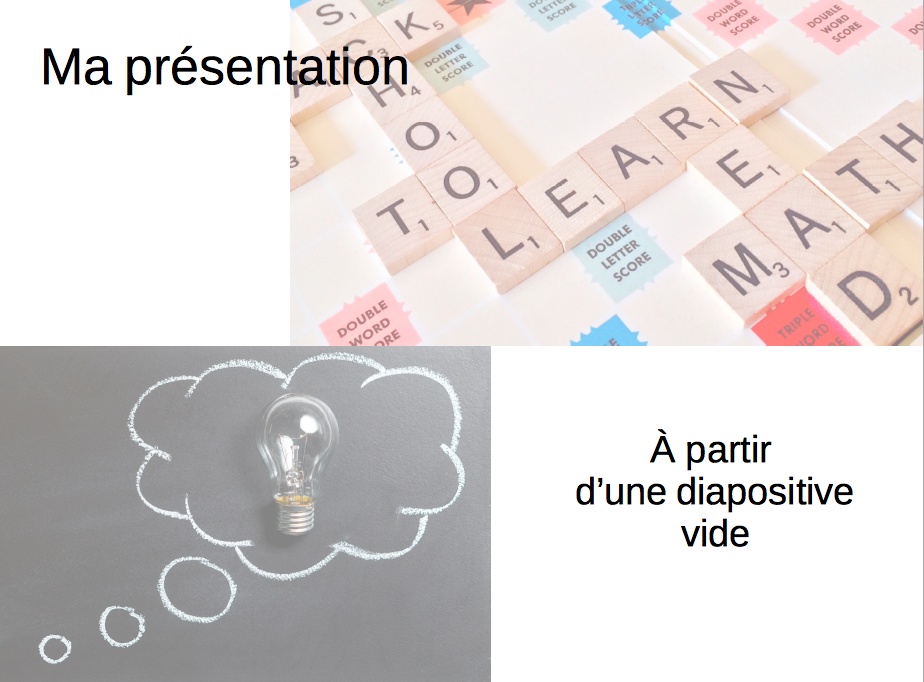
\includegraphics[angle=0,width=.75\textwidth]{./images/presentation/Impress_07DiaSansFormat_10}
\uneimageici{./images/presentation/Impress_07DiaSansFormat_10}{.4\textwidth}

%\end{minipage}\hfill%

\subsubsection{Insérer un texte dans une diapositive}\index{Impress!Insérer un texte}\index{Texte, insérer (Impress)}\label{Presentation1texte}
%\begin{minipage}[c]{.38\textwidth}

%\end{minipage}

\vspace{1em}

La première étape est de sélectionner une diapositive vide dans le choix de modèles comme montré dans la figure ci-dessous.



\uneimageici{./images/presentation/Impress_07DiaSansFormat_02_OPP_crop}{.7\textwidth}

Pour ajouter du texte sur cette diapositive, il faut se rendre sous l'onglet \texttt{Insertion} \circled{1} et utiliser l'outil \texttt{Zone de texte} \circled{2}.

\uneimageici{./images/presentation/Impress_07DiaSansFormat_03_OPP_crop}{.8\textwidth}

Une fois la zone de texte posée, on peut immédiatement commencer à écrire dedans. Les options de mise en forme du texte se retrouvent dans l'onglet \texttt{Accueil} \circled{1}. Les poignées de saisie et de rotation permettent de modifier la taille et l'orientation de la zone de texte, comme s'il s'agissait d'une image \circled{2}.

\uneimageici{./images/presentation/Impress_07DiaSansFormat_04_OPP_crop}{.7\textwidth}

\vspace{1em}

En cliquant sur le cadre de l'espace de texte (mais pas sur les poignées de saisie), on peut ensuite le déplacer sur la diapositive. 

\vspace{1em}

Pour modifier la taille des caractères, deux possibilités :
\begin{itemize}
\item sélectionner toute la zone de texte en cliquant sur le cadre (\circled{1} sur la figure ci-dessous à gauche) puis choisir la taille des caractères (\circled{2}) ; 
\item sélectionner le texte uniquement (figure à droite ci-dessous), puis choisir la taille des caractères.
\end{itemize}

\deuximagesici{./images/presentation/Impress_07DiaSansFormat_03_OPP2_crop}{.9\textwidth}
	      {./images/presentation/Impress_07DiaSansFormat_04_OPP2_crop}{.9\textwidth}


\subsubsection{Insérer une image dans une diapositive}\index{Impress!Insérer une image}\index{Image, insérer (Impress)}\label{Presentation1image}

Pour insérer une image, il faut se rendre dans l'onglet \texttt{Accueil} \circled{1}, puis cliquer sur le bouton \texttt{Image} \circled{2}, ce qui ouvre une liste de sources possibles pour l'image. Choisir \texttt{Cet appareil...} \circled{3} pour importer directement une image enregistrée sur l'ordinateur. Les autres options permettent de choisir des images autre part.

\uneimageici{./images/presentation/Impress_07DiaSansFormat_08_OPP_crop}{.7\textwidth}



\subsubsection{Définir une image d'arrière-plan}\index{Impress!Image d'arrière-plan}\index{Image d'arrière-plan (Impress)}\label{Presentation1imageFond}

Pour ajouter une image en arrière-plan de la diapositive, c'est-à-dire une image qui occupe tout le fond de la diapositive, il faut accéder au menu de mise en forme de l'arrière-plan. Pour cela, sous l'onglet \texttt{Création} \circled{1}, cliquer sur \texttt{Mise en forme de l'arrière-plan} \circled{2}. Le \texttt{Remplissage uni} \circled{3} permet de choisir une couleur à utiliser comme fond, et l'option \texttt{Image à partir d'un fichier} \circled{4} permet d'importer une image qui sera utilisée comme arrière-plan.

\uneimageici{./images/presentation/imageAPmenu_OPP_crop}{.7\textwidth}


Pour supprimer une image d'arrière-plan (ou tout autre arrière-plan personnalisé), il faut se rendre dans le même menu de mise en forme d'arrière-plan et cliquer sur \texttt{Arrière-plan uni} et choisir le blanc : la diapositive aura à nouveau un arrière-plan blanc uni. 



\subsubsection{Utiliser les animations}\index{Impress!Animations}\index{Animation (Impress)}\label{Presentation1effets}

Les animations permettent par exemple de faire afficher une diapositive en plusieurs temps : certaines parties de la diapositive arrivant après d'autres ou disparaissant avant le reste de la diapositive. Mais attention, il faut faire un usage parcimonieux des animations : les diaporamas en contenant trop sont souvent pénibles à suivre !

La première étape pour ajouter une animation est de sélectionner l'élément de la diapositive devant être affiché après les autres, comme par exemple un texte \circled{1}. Ensuite, il faut se rendre dans l'onglet \texttt{Animations} \circled{2} et choisir l'animation que l'on souhaite utiliser. Il existe plusieurs types d'animations, comme les effets d'entrée \circled{3}, les effets d'accentuation \circled{4} ou les effets de sortie \circled{5}. Pour une animation de texte arrivant sur la diapositive, c'est un effet d'entrée qu'il faut choisir.

\uneimageici{./images/presentation/Impress_08_Transitions_01_OPP_crop}{.6\textwidth}

Si une diapositive doit contenir plus d'une animation, il faut décider dans quel ordre elles ont lieu. Par exemple, un texte doit apparaitre avant une image, et on veut ensuite retirer l'image pour ajouter encore plus de texte. Pour réaliser ce genre de séquence, il faut d'abord voir comment les animations sont ordonnées : grâce à une numérotation apparaissant dans des rectangles à côté des éléments affectés \circled{1}. En sélectionnant un de ces éléments, on peut cliquer sur les boutons \texttt{Déplacer avant} et \texttt{Déplacer après} \circled{2} pour avancer ou reculer cette animation dans la liste.

\uneimageici{./images/presentation/Impress_08_Transitions_02_OPP_crop}{.6\textwidth}

Pour supprimer une animation, il faut sélectionner l'élément de la présentation qui a une présentation que l'on désire retirer et choisir \texttt{Aucune}.


Si on veut voir les animations des diapositives, on peut lancer le diaporama. Pour faire cela, il faut utiliser l'un des deux boutons suivants:
\begin{itemize}
	\item Le petit bouton Diaporama, en bas à droite, lance le diaporama à partir de la diapositive à l'écran. \circled{1}
	\item Dans l'onglet \texttt{Diaporama} \circled{2}, le bouton \texttt{À partir de la diapositive actuelle} permet également de lancer le diaporama à partir de ce pointr. \circled{3}
	\item Dans le même onglet, le bouton \texttt{À partir du début} permet de lancer le diaporama depuis le début. \circled{4}
\end{itemize}

\uneimageici{./images/presentation/Impress_08_Transitions_04_OPP_crop}{\textwidth}

En mode diaporama, il existe de nombreux moyens de naviguer entre les diapositives:
\begin{itemize}
	\item Les touches de déplacement $\leftarrow$, $\uparrow$, $\rightarrow$ et $\downarrow$ ;
	\item La touche espace ;
	\item Les touches n (comme "next", suivant) et p (comme "previous", précédent) ;
	\item Un clic de souris ;
	\item Le menu d'options se révélant en bas à gauche de la présentation. Il permet notamment d'atteindre directement une diapositive spécifique.	\circled{5}
\end{itemize}

Enfin, on peut quitter un diaporama avant d'être arrivé au bout grâce à la touche Esc.


\subsubsection{Ajouter des notes de présentation}\index{Impress!Notes de présentation}\index{Notes de présentation (Impress)}\label{Presentation1notes}


%\begin{minipage}[c]{.68\textwidth}
Il est possible d'ajouter des \emph{\og notes \fg} associées aux diapositives. Ces notes servent d'aide au présentateur et n'apparaissent pas à l'écran lors de la présentation (sauf sur l'écran secondaire s'il y en a un).

Pour ajouter des notes à une diapositive, sélectionner la diapositive à laquelle on veut les ajouter et cliquer sur le bouton \texttt{Notes}, en bas de l'écran.

\uneimageici{./images/presentation/Impress_06Notes_01_OPP_crop}{.4\textwidth}

Apparait alors en bas de l'écran un espace de texte dans lequel vous pouvez rédiger vos notes.

\uneimageici{./images/presentation/Impress_06Notes_02_OPP_crop}{.7\textwidth}


\subsubsection{Imprimer une présentation et ses notes}\index{Impress!Imprimer}\index{Imprimer (Impress)}\label{Presentation1export}

Pour imprimer les diapositives et les notes associées, il faut se rendre dans le menu \texttt{Fichier} et choisir \texttt{Imprimer...}. \circled{1} Il faut ensuite choisir ce qu'on désire imprimer.

\begin{itemize}
	\item La première option imprime une diapositive par page \circled{2} ;
	\item La deuxième fait de même mais ajoute les notes aux côtés des diapositives \circled{3} ;
	\item La dernière imprime trois diapositives par page avec de la place pour y écrire des commentaires. \circled{4}
\end{itemize}

\uneimageici{./images/presentation/Impress1_impression01_OPP_crop}{.5\textwidth}

Quelle que soit l'option sélectionnée, un fichier PDF contenant ce qui doit être imprimé est préparé. Il suffit de l'ouvrir avant de pouvoir l'imprimer normalement. Pour ce faire, cliquer sur les touches \texttt{Cmd + P} pour ouvrir la fenêtre d'impression. Là, on peut choisir le nombre de copies, l'organisation des pages, et toutes les autres options d'impression. Pour lancer l'impression, cliquer sur le bouton \texttt{Imprimer}, en bas à droite de la fenêtre.

\uneimageici{./images/presentation/Impress1_impression02_OPP_crop}{.5\textwidth}


\subsubsection{Exporter une présentation et ses notes au format PDF}\index{Impress!Exporter au format PDF}\index{Exporter au format PDF (Impress)}\label{Presentation1exportPDF}


Pour exporter une présentation au format PDF, il faut procéder comme indiqué plus haut, mais à la fenêtre d'impression, au lieu de cliquer sur \texttt{Imprimer}, il faut choisir le bouton \texttt{PDF}, en bas à gauche. On peut alors enregistrer le fichier PDF contenant la présentation.

\uneimageici{./images/presentation/Impress1_impression03_OPP_crop}{.45\textwidth}


\vfill
\phantom{rien}






